\pagestyle{headings}
\chapter{Interval Estimation} \label{chp 7}
\thispagestyle{fancy}

\subsection*{Introduction: Quantifying Estimation Error}
The techniques of point estimation which we've developed over the last chapter are useful when a single well justified guess at the value of an unknown parameter is called for. However, point estimates often do not provide sufficient information to inform important decisions.
\par
Suppose a report on labor in Canada states that the unemployment rate has risen from 6.8\% in June 2016 to 7.1\% in June 2017. Each of these numbers is a point estimate derived from a sample, and therefore each represents a single observation drawn from a sampling distribution.
\par
The naive interpretation of the report on labor is that the unemployment rate has gone up, but those two figures stated depend not only on the actual state of the labor market, but also on a random result of a sampling process. It's possible that the unemployment rate in Canada in June 2016 was in fact 7.0\%, we just happened to draw a sample which resulted in an underestimate, and perhaps the unemployment rate in Canada in June 2017 was in fact 6.9\%, we just happened to draw a sample which resulted in an overestimate.
\par
When providing an estimate of an unknown parameter, we would like to be able to quantify the uncertainty inherent in the process that produced it. In our example, instead of stating (probably falsely) that the unemployment rate in Canada in June 2016 was 6.8\%, it would be much more useful to say that with 95\% confidence, the unemployment rate in Canada in June 2016 was between, say, 6.6\% and 7.0\%. This way when we compare two statistics, we'll be better able to assess whether the difference between those two values is significant or not.
\ \\
\ \\
\ \\

\section{The Law of Large Numbers}

The law of large numbers is one of the cornerstones of statistical inference. This is a mathematically precise statement of the fairly intuitive principle that if we take a larger and larger SRS of values, the mean in our sample tends to become closer and closer to the mean in the population. This principle is often informally referred to as `regression to the mean'.

\begin{thm} (Weak Law of Large Numbers)\index{Law of Large Numbers} Suppose that $X$ is a random variable with mean $\mu$ and standard deviation $\sigma$. If $X_1, X_2, \dots \, , X_n$ is a SRS of values of $X$ taken with replacement, then for any $\epsilon > 0$,
\eqnsgap{\lim_{n \to \infty} P\left(\left|\frac{X_1+X_2+\,\cdots\,+X_n}{n} - \mu \right| \geq \epsilon \right) = 0}
\end{thm}
\par
In other words, for any interval containing $\mu$, no matter how tiny it might be, the probability of obtaining a sample whose mean is outside that interval approaches zero as the sample size approaches infinity. This result holds for any population distribution whose expected value and standard deviation are defined.
\par
\vspace{1em}
\begin{pf} Let $\xbar = \frac{X_1+X_2+\,\cdots\,+X_n}{n}$. Our sample $X_1, X_2, \dots \,, X_n$ is a SRS, so each $X_i$ has the same distribution as $X$, hence $E(X_i) = E(X) = \mu$. By linearity of expectation,
\eqnspar{E(\xbar) &= E\left(\frac{X_1+X_2+\,\cdots\,+X_n}{n}\right) \\
&= \frac{1}{n}(E(X_1)+E(X_2)+\,\cdots\,+E(X_n))  \\
&= \frac{1}{n}(n\mu) = \mu.}
\par
\noindent We can also obtain a simple expression for the variance of $\xbar$ by making use of the properties of variance we demonstrated in Theorem \ref{VarianceIndependentSum} and \ref{VarianceLinearity}.
\eqns{\Var(\xbar) &= \Var\left(\frac{X_1+X_2+\,\cdots\,+X_n}{n}\right) \\
&= \frac{1}{n^2}\Var(X_1 + X_2 + \, \cdots \, + X_n) \\
&=\frac{1}{n^2}(\Var(X_1) + \Var(X_2) + \, \cdots \, + \Var(X_n)) \\
&=\frac{1}{n^2}(n\sigma^2) = \frac{\sigma^2}{n}}
\par
\noindent
Thus, the mean of $\xbar$ is $\mu$, and the standard deviation of $\xbar$ is $\sqrt{\frac{\sigma^2}{n}} = \frac{\sigma}{\sqrt{n}}$.
\par
\noindent Our goal is to show that $\xbar$ can't stray too far from it's mean, $\mu$, and we have a tool for bounding the values a random variable can take: Chebyshev's Inequality (Theorem \ref{ChebyshevsInequality}). Applying the inequality to $\xbar$, we have that for any $k > 0$,

\eqns{P\bigr(\xbar \in (\mu - k\textstyle\frac{\sigma}{\sqrt{n}}, \, \mu + k\frac{\sigma}{\sqrt{n}})\bigr) &\geq 1 - \frac{1}{k^2} \\
P\bigr(\xbar \not\in (\mu - k\textstyle\frac{\sigma}{\sqrt{n}}, \, \mu + k\frac{\sigma}{\sqrt{n}})\bigr) &\leq \frac{1}{k^2}.}
\vspace{0.5em}
\par
\noindent Now given any $\epsilon > 0$, take $k = \frac{\epsilon\sqrt{n}}{\sigma}$. Isolating $\frac{1}{k^2}$ in this equation yields $\frac{1}{k^2} = \frac{\sigma^2}{\epsilon^2n}$, and isolating $\epsilon$ gives $\epsilon = k\frac{\sigma}{\sqrt{n}}$, so we can rewrite the inequality above as
\eqns{P\bigr(\xbar \not\in (\mu - \epsilon, \, \mu + \epsilon)\bigr) &\leq \frac{\sigma^2}{\epsilon^2n} \\
P\left(\left|\frac{X_1 + X_2 + \, \cdots \, + X_n}{n} - \mu \right| \geq \epsilon \right) &\leq \frac{\sigma^2}{\epsilon^2n}.}
\par
\noindent To complete the argument, observe that $\frac{\sigma^2}{\epsilon^2n}$ approaches zero as $n \to \infty$.
\end{pf}
\par
The results concerning the mean and standard deviation of $\overline{X}$ we obtained before applying Chebyshev's Inequality are significant in their own right, so we'll restate them below.
\begin{cor}\label{StandardErrorOfMean} Suppose $X_1, X_2, \dots\, , X_n$ is a SRS drawn from a population with mean $\mu$ and standard deviation $\sigma$, and let $\xbar = \frac{X_1+ X_2+ \cdots + X_n}{n}$. The mean and standard deviation of the sampling distribution of $\xbar$ are given by
\eqnsgap{\boxed{\ \muxbar = \mu \qquad \sigmaxbar = \frac{\sigma}{\sqrt{n}}\ }}
\end{cor}
\par
The strong law of large numbers, given below, is also a statement that the mean of a SRS will converge to the population mean as the sample size approaches infinity, but the notion of convergence is slightly different. This alternate formulation is more difficult to prove, but can be easier to apply.

\begin{thm} (Strong Law of Large Numbers) Suppose that $X$ is a random variable with mean $\mu$. If $X_1, X_2, \dots \, , X_n$ is a SRS of values of $X$ taken with replacement, then
\eqnsgap{P\left( \lim_{n \to \infty} \frac{X_1+X_2+\,\cdots\,+X_n}{n} = \mu \right) = 1}
\end{thm}

\par
One of the more entertaining consequences of the strong law of large numbers is the classic result below.

\begin{examp} (Infinite Monkey Theorem) If an immortal monkey at a typewriter presses keys at random for eternity, show that the monkey will eventually produce the complete works of Shakespeare.
\par
\noindent Consider the infinite sequence of keys the monkey types. Break that sequence up into infinitely many disjoint blocks of length $N$, where $N$ is the number of key presses required to produce the complete works of Shakespeare. Let $A_i$ be the event `the $i^{th}$ block of length $N$ is an exact reproduction of the complete works of Shakespeare', and let $X_i$ be a random variable defined by
\eqns{X_i = \left\{
\begin{array}{cl}
      1 & \text{if } A_i \text{\ occurs}  \\
      0 & \text{if } A_i \text{\ doesn't occur} \\ \end{array}
\right.}
\par
\noindent Assuming the monkey selects each key uniformly at random, without any regard to previous choices, we have $P(X_i = 1) = (\frac{1}{k})^N$ and $P(X_i = 0) = 1 - (\frac{1}{k})^N$, where $k$ is the number of keys on the typewriter. Furthermore, the events $A_1, A_2, \dots \,, A_n$ form an independent sequence since the blocks of length $N$ do not overlap.
\par
\noindent Therefore, the random variables $X_i$ are independent and identically distributed. In other words, they form a SRS of $n$ values from a random variable $X$ which takes value one with probability $(\frac{1}{k})^N$ and zero with probability $1 - (\frac{1}{k})^N$.
\par
\noindent The expected value of $X$ is $\mu = E(X) = 1 \cdot (\frac{1}{k})^N + 0 \cdot (1- (\frac{1}{k})^N) = (\frac{1}{k})^N$. Thus, by the strong law of large numbers,
\eqns{P\left(\lim_{n \to \infty} \frac{X_1+X_2+\,\cdots\,+X_n}{n} = \left(\frac{1}{k}\right)^N \right) = 1}
\par
\noindent Note that $\left(\frac{1}{k}\right)^N \neq 0$, so with probability one, $\lim_{n \to \infty} \frac{X_1+X_2+\,\cdots\,+X_n}{n}$ is not zero. This means that the sum $X_1+X_2+\,\cdots\,+X_n \to \infty$ as $n \to \infty$, since if this sum was bounded by some constant $c$, then $\frac{X_1+X_2+\,\cdots\,+X_n}{n} \leq \frac{c}{n} \to 0$. Therefore, we have $X_i = 1$ for infinitely many $i$, so with probability one, not only will the monkey produce the complete works of Shakespeare, it will do so infinitely many times!
\end{examp}
\par
The law of large numbers is frequently misunderstood. Consider a scenario in which a fair coin is repeatedly flipped. The law of large numbers states that as the number of flips grows larger and larger, the proportion of heads will converge to $\frac{1}{2}$ with probability one.
\par
If the first five flips all result in tails, it might seem reasonable to use the law of large numbers to argue that the coin is `due for heads', and so heads must now be more likely than tails, since the proportion of heads must converge to $\frac{1}{2}$. This is known as the gambler's fallacy\index{Gambler's Fallacy}.
\par
The key point is that as the number of flips grows very large, the influence of the first five flips on the proportion of heads becomes less and less significant. Suppose that after the first five flips, all of which are tails, heads and tails simply alternate, beginning with heads. After ten flips, the proportion of heads is $\frac{3}{10} = 30\%$, after one hundred flips, it's $\frac{48}{100} = 48\%$, and after one thousand flips, it's $\frac{498}{1000} = 49.8\%$. The coin does not need to become biased towards heads to bring the proportion of heads closer to $\frac{1}{2}$. After many flips, the initial streak of five tails simply becomes less and less significant.

%\subsection*{Convergence of the Empirical Distribution}
%Suppose that we take a random sample of $n$ values from some population, and %consider the distribution of values in our sample.
%
%\begin{examp}Let $X \sim Exponential(\frac{1}{2})$. A sample of $n$ values was drawn from this distribution, and the distribution of values in the sample is shown as a histogram. This was done for $n=10$, $n=100$, and $n=1000$. Along with each histogram, the pdf $f_X$ is shown as a dashed curve.
%
%\begin{center}
%    \begin{minipage}{.5\textwidth}
%        \centering
%  \begin{tikzpicture}[scale = 0.6]
%       \begin{axis}[title = {$X \sim Exponential(\frac{1}{2})$}, ymin=0,ymax=0.6,xmin=-0.0025, xmax = 6.2, xtick = {0,1,2,3,4,5,6}, ytick = {1}, area style]
%       \addplot+[ybar interval,mark=no] plot coordinates {(0,0.44) (0.5,0.4) (1,0.16) (1.5,0.22) (2,0.24) (2.5,0.1) (3,0.14) (3.5,0.06) (4,0.06) (4.5,0.02) (5,0.02) (5.5,0.02) (6,0)};
%       \addplot[dashed,domain=0:6.5,black] {0.5*e^(-0.5*x)};
%       \draw[very thick, blue, -] (axis cs:0,0) -- (axis cs:0,2);
%    \end{axis}
%    \end{tikzpicture}
%    \end{minipage}%
%    \begin{minipage}{0.5\textwidth}
%        \centering
%  \begin{tikzpicture}[scale = 0.6]
%       \begin{axis}[title = {$X \sim Exponential(\frac{1}{2})$}, ymin=0,ymax=0.6,xmin=-0.0025, xmax = 6.2, xtick = {0,1,2,3,4,5,6}, ytick = {1}, area style]
%       \addplot+[ybar interval,mark=no] plot coordinates {(0,0.398) (0.5,0.342) (1,0.276) (1.5,0.226) (2,0.148) (2.5,0.144) (3,0.112) (3.5,0.088) (4,0.076) (4.5,0.04) (5,0.026) (5.5,0.022) (6,0.024)};
%       \addplot[dashed,domain=0:6.5,black] {0.5*e^(-0.5*x)};
%       \draw[very thick, blue, -] (axis cs:0,0) -- (axis cs:0,2);
%    \end{axis}
%    \end{tikzpicture}
%\end{minipage}
%\end{center}
%
%\end{examp}

%Formally, if $X_1, X_2, \dots, X_n$ are the $n$ sample values, let $S_n$ be a random variable whose value is given by uniformly selecting an integer $i$ between $1$ and $n$ inclusive, and letting $S_n = X_i$, so that $S_n$ represents a randomly selected value in our sample.

\section{The Central Limit Theorem}

In the last section, two extremely important general results were established. We found expressions for the mean and standard deviation of the sampling distribution of $\xbar$ (given in Corollary \ref{StandardErrorOfMean}) which hold for any random variable $X$ whose mean $\mu$ and standard deviation $\sigma$ are defined, and we showed the sample mean will converge to the population mean as the sample size grows without bound.
\par
In other words, the sampling distribution of $\xbar$ will cluster tighter around the population mean $\mu$ as the sample size grows larger and samples which have sample means far from $\mu$ become more and more rare. 
\par
What about the shape of the sampling distribution of $\xbar$? What happens as the sample size increases? Consider the population distribution $X \sim Exponential(\frac{1}{2})$. Let's approximate the sampling distribution of $\xbar$ by taking ten thousand SRSs and calculating their means. With a sample size of one, the result should look just like the population distribution, since the mean of a single observation is just that observation itself.

\begin{center}
    \begin{minipage}{.5\textwidth}
        \centering
  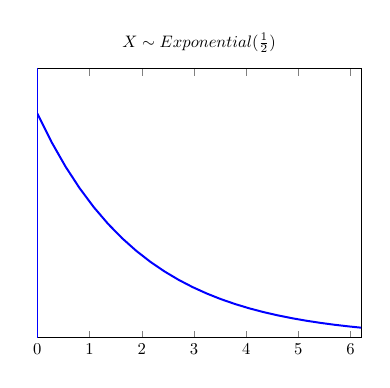
\begin{tikzpicture}[scale = 0.6]
       \begin{axis}[title = {$X \sim Exponential(\frac{1}{2})$}, ymin=0,ymax=0.6,xmin=-0.0025, xmax = 6.2, xtick = {0,1,2,3,4,5,6}, ytick = {1}]
       \addplot[very thick,domain=0:6.5,blue] {0.5*e^(-0.5*x)};
       \draw[very thick, blue, -] (axis cs:0,0) -- (axis cs:0,2);
    \end{axis}
    \end{tikzpicture}
    \end{minipage}%
    \begin{minipage}{0.5\textwidth}
        \centering
  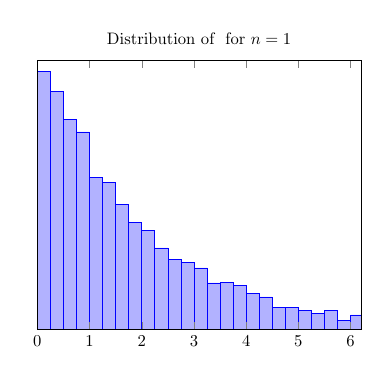
\begin{tikzpicture}[scale = 0.6]
\begin{axis}[title = {Distribution of $\xbar$ for $n=1$}, ymin=0,ymax=1200,xmin=-0.0025, xmax = 6.2, xtick = {0,1,2,3,4,5,6}, ytick = {1500}, area style]
\addplot+[ybar interval,mark=no] plot coordinates {(0,1153) (0.25,1063) (0.5,939) (0.75,882) (1,678) (1.25,655) (1.5,557) (1.75,479) (2,443) (2.25,364) (2.5,313) (2.75,298) (3,275) (3.25,208) (3.5,211) (3.75,198) (4,161) (4.25,146) (4.5,99) (4.75,99) (5,86) (5.25,73) (5.5,86) (5.75,41) (6,65) (6.25,54)};
\end{axis}
\end{tikzpicture}
\end{minipage}
\end{center}

What happens when we increase the sample size to two? Let's take ten thousand samples, each consisting of two independent observations of $X \sim Exponential(\frac{1}{2})$, and compute the mean of each sample. The resulting distribution is given below.

\begin{center}
    \begin{minipage}{.5\textwidth}
        \centering
  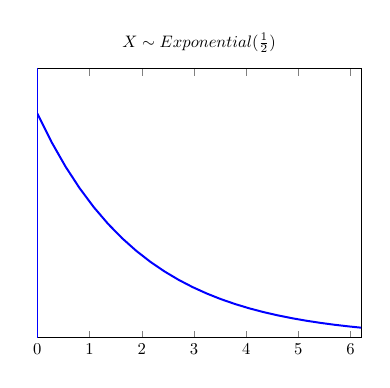
\begin{tikzpicture}[scale = 0.6]
       \begin{axis}[title = {$X \sim Exponential(\frac{1}{2})$}, ymin=0,ymax=0.6,xmin=-0.0025, xmax = 6.2, xtick = {0,1,2,3,4,5,6}, ytick = {1}]
       \addplot[very thick,domain=0:6.5,blue] {0.5*e^(-0.5*x)};
       \draw[very thick, blue, -] (axis cs:0,0) -- (axis cs:0,2);
    \end{axis}
    \end{tikzpicture}
    \end{minipage}%
    \begin{minipage}{0.5\textwidth}
        \centering
  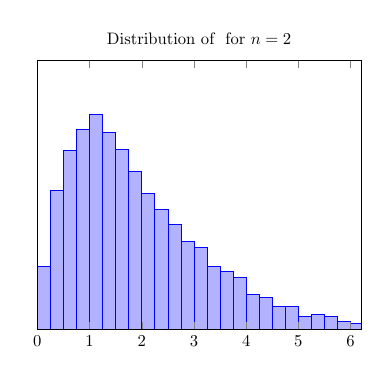
\begin{tikzpicture}[scale = 0.6]
\begin{axis}[title = {Distribution of $\xbar$ for $n=2$}, ymin=0,ymax=1200,xmin=-0.0025, xmax = 6.2, xtick = {0,1,2,3,4,5,6}, ytick = {1500}, area style]
\addplot+[ybar interval,mark=no] plot coordinates {(0,282) (0.25,620) (0.5,801) (0.75,894) (1,959) (1.25,880) (1.5,803) (1.75,706) (2,608) (2.25,537) (2.5,469) (2.75,394) (3,366) (3.25,283) (3.5,260) (3.75,231) (4,158) (4.25,142) (4.5,103) (4.75,105) (5,57) (5.25,67) (5.5,57) (5.75,37) (6,27) (6.25,36)};
\end{axis}
\end{tikzpicture}
\end{minipage}
\end{center}

If we continue to increase the sample size, taking ten thousand random samples of larger and larger sizes from the same population distribution, and computing the mean of each, how will the distribution of these means change?

\begin{center}
    \begin{minipage}{.5\textwidth}
        \centering
  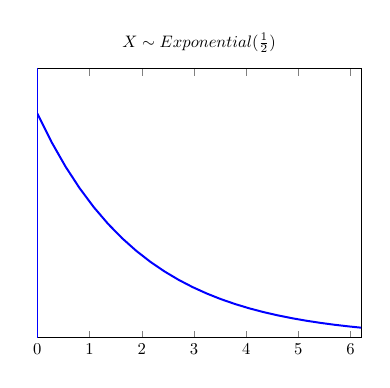
\begin{tikzpicture}[scale = 0.6]
       \begin{axis}[title = {$X \sim Exponential(\frac{1}{2})$}, ymin=0,ymax=0.6,xmin=-0.0025, xmax = 6.2, xtick = {0,1,2,3,4,5,6}, ytick = {1}]
       \addplot[very thick,domain=0:6.5,blue] {0.5*e^(-0.5*x)};
       \draw[very thick, blue, -] (axis cs:0,0) -- (axis cs:0,2);
    \end{axis}
    \end{tikzpicture}
    \end{minipage}%
    \begin{minipage}{0.5\textwidth}
        \centering
  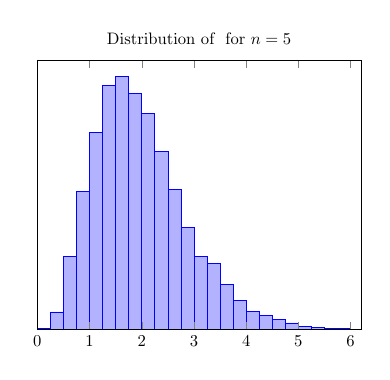
\begin{tikzpicture}[scale = 0.6]
\begin{axis}[title = {Distribution of $\xbar$ for $n=5$}, ymin=0,ymax=1300,xmin=-0.0025, xmax = 6.2, xtick = {0,1,2,3,4,5,6}, ytick = {1500}, area style]
\addplot+[ybar interval,mark=no] plot coordinates {(0,4) (0.25,85) (0.5,355) (0.75,668) (1,954) (1.25,1180) (1.5,1224) (1.75,1140) (2,1045) (2.25,861) (2.5,678) (2.75,495) (3,354) (3.25,318) (3.5,218) (3.75,139) (4,89) (4.25,67) (4.5,49) (4.75,32) (5,17) (5.25,11) (5.5,4) (5.75,6) (6,2) (6.25,2)};
\end{axis}
\end{tikzpicture}
\end{minipage}
\end{center}

\begin{center}
    \begin{minipage}{.5\textwidth}
        \centering
  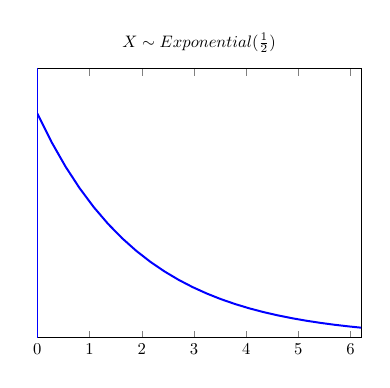
\begin{tikzpicture}[scale = 0.6]
       \begin{axis}[title = {$X \sim Exponential(\frac{1}{2})$}, ymin=0,ymax=0.6,xmin=-0.0025, xmax = 6.2, xtick = {0,1,2,3,4,5,6}, ytick = {1}]
       \addplot[very thick,domain=0:6.5,blue] {0.5*e^(-0.5*x)};
       \draw[very thick, blue, -] (axis cs:0,0) -- (axis cs:0,2);
    \end{axis}
    \end{tikzpicture}
    \end{minipage}%
    \begin{minipage}{0.5\textwidth}
        \centering
  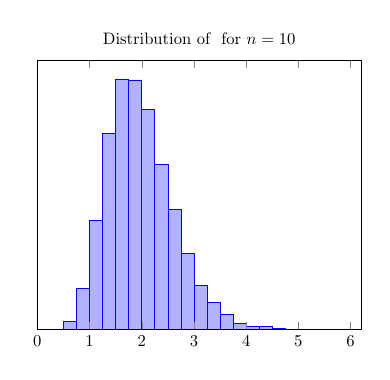
\begin{tikzpicture}[scale = 0.6]
\begin{axis}[title = {Distribution of $\xbar$ for $n=10$}, ymin=0,ymax=1750,xmin=-0.0025, xmax = 6.2, xtick = {0,1,2,3,4,5,6}, ytick = {2000}, area style]
\addplot+[ybar interval,mark=no] plot coordinates {(0,0) (0.25,1) (0.5,55) (0.75,269) (1,709) (1.25,1275) (1.5,1631) (1.75,1624) (2,1434) (2.25,1073) (2.5,782) (2.75,493) (3,288) (3.25,175) (3.5,102) (3.75,42) (4,22) (4.25,18) (4.5,5) (4.75,0) (5,2) (5.25,0) (5.5,0) (5.75,0) (6,0) (6.25,0)};
\end{axis}
\end{tikzpicture}
\end{minipage}
\end{center}

\begin{center}
    \begin{minipage}{.5\textwidth}
        \centering
  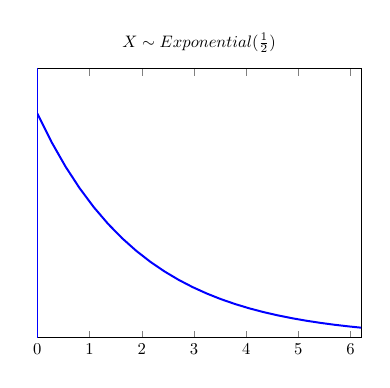
\begin{tikzpicture}[scale = 0.6]
       \begin{axis}[title = {$X \sim Exponential(\frac{1}{2})$}, ymin=0,ymax=0.6,xmin=-0.0025, xmax = 6.2, xtick = {0,1,2,3,4,5,6}, ytick = {1}]
       \addplot[very thick,domain=0:6.5,blue] {0.5*e^(-0.5*x)};
       \draw[very thick, blue, -] (axis cs:0,0) -- (axis cs:0,2);
    \end{axis}
    \end{tikzpicture}
    \end{minipage}%
    \begin{minipage}{0.5\textwidth}
        \centering
  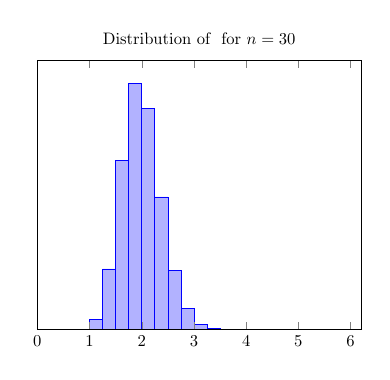
\begin{tikzpicture}[scale = 0.6]
\begin{axis}[title = {Distribution of $\xbar$ for $n=30$}, ymin=0,ymax=2900,xmin=-0.0025, xmax = 6.2, xtick = {0,1,2,3,4,5,6}, ytick = {3000}, area style]
\addplot+[ybar interval,mark=no] plot coordinates {(0,0) (0.25,0) (0.5,0) (0.75,6) (1,108) (1.25,653) (1.5,1826) (1.75,2653) (2,2385) (2.25,1430) (2.5,636) (2.75,230) (3,59) (3.25,12) (3.5,2) (3.75,0) (4,0) (4.25,0) (4.5,0) (4.75,0) (5,0) (5.25,0) (5.5,0) (5.75,0) (6,0) (6.25,0)};
\end{axis}
\end{tikzpicture}
\end{minipage}
\end{center}
\par
Each of the sampling distributions has mean $\muxbar = 2$, the same as the population distribution, and the standard deviation becomes smaller and smaller as $n$ increases, as Corollary \ref{StandardErrorOfMean} assures us it will (since $\sigmaxbar = \sigma / \sqrt{n} \to 0$ as $n \to \infty$).
\par
Moreover, there is a striking trend in the shapes of the sampling distributions. As the sample size increases, the distribution looks less like an exponential distribution, and more like a normal distribution (albeit a narrow one).
\par
It's not a coincidence that this occurred in our particular example. In fact, this occurs for almost \emph{any} population! This is a hugely important result, and it's why the normal distribution plays such a central role in statistics. If some quantity is obtained by averaging a random sample, and the sample size is large enough, then we know that the sampling distribution it was drawn from must be approximately normal \emph{regardless of the shape of the population distribution!}
\par
\begin{thm} (Central Limit Theorem)\index{Central Limit Theorem}\label{CLT} Let $X$ be a random variable with a well-defined mean $\mu$ and standard deviation $\sigma$, and let $\xbar$ denote the mean of a simple random sample of $n$ values drawn from the distribution of $X$. Then as the sample size $n$ grows larger, the sampling distribution of $\xbar$ becomes better approximated by $Normal(\muxbar,\sigmaxbar)$.
\end{thm}
\par
The conclusion of this theorem is written here in very informal language. To make it more precise, we would need to decide on a way to measure the difference between two random variables, so the theorem above could state that this difference vanishes as $n \to \infty$. For details see \cite{Bertsekas} or \cite{DevoreBerk}.

\begin{examp}\label{CLTExamp}Twenty numbers in the interval $[0,1]$ are independently chosen uniformly at random. What is the probability their sum is higher than eight?
\par
\noindent In order to use the central limit theorem, we need to formulate this question in terms of the mean of a sample. In this case, we have a sample of $n=20$ values drawn from $X \sim Uniform([0,1])$. Observe that
\eqnspar{X_1 + X_2 + \cdots + X_{20} > 8 \ \ \rightarrow \ \  \frac{X_1 + X_2 + \cdots + X_{20} }{20} > \frac{8}{20} = \frac{2}{5}.}
\par
\noindent Thus, to answer this question, we need to find the probability of obtaining a sample of twenty values with a mean $\xbar$ higher than $\frac{2}{5}$. Using Corollary \ref{StandardErrorOfMean} and Proposition \ref{UniformVariance} The mean and standard deviation of $\xbar$ are given by
\eqns{\muxbar = \mu = \frac{1}{2} \ \  \text{and} \ \  \sigmaxbar = \frac{\sigma}{\sqrt{n}} = \frac{\sqrt{\frac{1}{12}(1-0)^2}}{\sqrt{20}} = \frac{1}{\sqrt{240}} \simeq 0.0645}
\par
\noindent The central limit theorem states that the distribution of $\xbar$ can be approximated by $Normal(0.5, 0.0645)$, so the probability of obtaining a sample with $\xbar$ higher than $\frac{2}{5} = 0.4$ can be calculated as follows.

\eqns{z = \frac{\xbar - \muxbar}{\sigmaxbar} = \frac{0.4 - 0.5}{0.0645} = \frac{-0.1}{0.0645} \simeq -1.55}

\vspace{-1em}
\begin{center}
    \begin{minipage}{.5\textwidth}
        \centering
  \eqns{P(\xbar > \textstyle\frac{2}{5}) &= P(Z > -1.55) \\ &= 1 - P(Z \leq -1.55) \\ &= 1 - 0.0603 \\ &= 0.9397 \simeq 94\%}
  \vspace{1.25em}
    \end{minipage}%
    \begin{minipage}{0.5\textwidth}
        \centering
   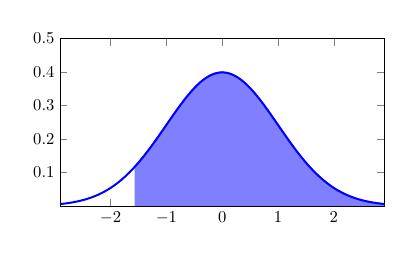
\begin{tikzpicture}[scale = 0.6]
       \begin{axis}[unit vector ratio=1 6 1, ymin=0,ymax=0.5,xmin=-2.9, xmax = 2.9, xtick = {-2,-1,0,1,2}, ytick = {0.1,0.2,0.3,0.4,0.5}]
       \addplot[fill = blue, very thick,domain=-1.55:3,blue!50, samples=100] {0.3989*e^(-x^2/2)}\closedcycle;
       \addplot[very thick,domain=-3:3,blue, samples=100] {0.3989*e^(-x^2/2)};
       \addplot[domain=-3:3] {0};
    \end{axis}
    \end{tikzpicture}
\end{minipage}
\end{center}
\par
\noindent Note that the central limit theorem does not tell us how closely the distribution of $\xbar$ is approximated by $Normal(0.5,0.0645)$. Let's take ten thousand samples and plot the resulting sampling distribution for $\xbar$, along with the normal distribution given by the central limit theorem.
\par
\noindent
If the two distributions match well, then we'll know that our answer above is fairly accurate. If the sampling distribution is still far from being normal, then we'll have to disregard our answer.
\begin{center}
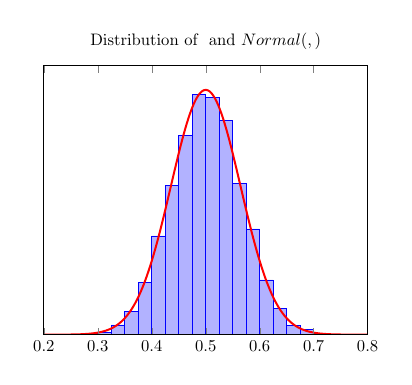
\begin{tikzpicture}[scale = 0.6]
\begin{axis}[title = {Distribution of $\xbar$ and $Normal(\muxbar,\sigmaxbar)$}, ymin=0,ymax=1700,xmin=0.2, xmax = 0.8, xtick = {0.2,0.3,0.4,0.5,0.6,0.7,0.8}, ytick = {3300}, area style]
\addplot+[ybar interval,mark=no] plot coordinates {(0,0) (0.025,0) (0.05,0) (0.075,0) (0.1,0) (0.125,0) (0.15,0) (0.175,0) (0.2,0) (0.225,0) (0.25,2) (0.275,6) (0.3,13) (0.325,61) (0.35,147) (0.375,328) (0.4,624) (0.425,942) (0.45,1257) (0.475,1520) (0.5,1499) (0.525,1355) (0.55,955) (0.575,668) (0.6,346) (0.625,167) (0.65,58) (0.675,34) (0.7,7) (0.725,0)};
\addplot[very thick,domain=0:1,red, samples=500] {250*6.185*e^((-(x - 0.5)^2)/(2*(1/240)))};
\end{axis}
\end{tikzpicture}
\end{center}
The distribution of $\xbar$ for samples of size twenty drawn from $X \sim Uniform([0,1])$ is extremely well approximated by a normal distribution, so we can be sure our answer is reasonably accurate.
\end{examp}

\subsection*{Sample Size}

The central limit theorem states that the sampling distribution of $\xbar$ will eventually become well approximated by a normal distribution once the sample size is large enough, but how large must our sample be so that when we use a normal distribution for calculations, as in the example above, our probability estimates will be accurate?
\par
The answer varies with the population distribution. Symmetric population distributions with thin tails (which decay exponentially) often yield sampling distributions for $\xbar$ which are very close to normal even for single digit sample sizes, while asymmetric population distributions with fat tails (which decay polynomially) can result in sampling distributions for $\xbar$ which don't look normal until the sample size becomes extremely large.
\par
As a rule of thumb, we'll use the guidelines below to determine if the sampling distribution of $\xbar$ is sufficiently close to normal that we can justify approximating it by a normal distribution.
\vspace{-0.5em}
\begin{enumerate}[(i)]
\item If the population distribution is normal, any sample size is fine.
\item If the population distribution is roughly symmetric and not fat-tailed, $n \geq 30$.
\item If the population distribution is significantly skewed or fat-tailed, $n \geq 50$.
\end{enumerate}
\par
There is nothing mathematically significant about these values, or similar values you'll find in other texts. We're simply establishing a clear (yet arbitrary) baseline. 
\par
In actual practice, to ensure the sampling distribution of $\xbar$ is sufficiently close to a normal distribution, statisticians either rigorously derive error bounds from some assumptions on the form of the population distribution, or use statistical software to take large numbers of samples from an educated guess at the population distribution and approximate the sampling distribution empirically, as was done to generate the graphics at the beginning of this section.
\begin{examp}
If a biased coin with a 55\% probability of heads is flipped thirty times, what is the probability that the number of heads observed in this sample is less than the number of tails?
\par
\noindent If we call a head a success, then we have a sample of 30 values $X_1,X_2\,\dots\,,X_{30}$ from $X \sim Bernoulli(0.55)$. If more tails than heads were observed, this means that more than half of the $X_i$ are zeros, so $\xbar = \frac{X_1 + X_2 + \cdots + X_{30}}{30} < \frac{15}{30} =0.5$.
\par
\noindent Note $X \sim Bernoulli(0.55)$ is roughly symmetric, so by the central limit theorem, the distribution of $\xbar$ is approximately normal for samples of $n = 30$ observations. The mean and standard deviation of the sampling distribution are given by 
\eqns{\muxbar = \mu = 0.55 \ \ \text{and} \ \  \sigmaxbar = \frac{\sigma}{\sqrt{n}} = \frac{\sqrt{p(1-p)}}{\sqrt{n}} = \frac{\sqrt{0.2475}}{\sqrt{30}} \simeq 0.091}
\par
\noindent Now we can calculate the probability of obtaining a sample mean $\xbar < 0.5$.

\eqns{z = \frac{\xbar - \muxbar}{\sigmaxbar} = \frac{0.5 - 0.55}{0.091} = \frac{-0.05}{0.091} \simeq -0.549}

\begin{center}
    \begin{minipage}{.5\textwidth}
        \centering
  \eqns{P(\xbar < 0.5) &= P(Z < -0.549) \\ &= 0.2905 \simeq 29\%}
  \vspace{1.25em}
    \end{minipage}%
    \begin{minipage}{0.5\textwidth}
        \centering
   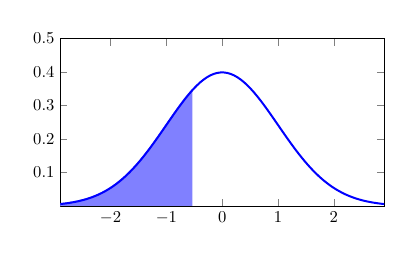
\begin{tikzpicture}[scale = 0.6]
       \begin{axis}[unit vector ratio=1 6 1, ymin=0,ymax=0.5,xmin=-2.9, xmax = 2.9, xtick = {-2,-1,0,1,2}, ytick = {0.1,0.2,0.3,0.4,0.5}]
       \addplot[fill = blue, very thick,domain=-3:-0.55,blue!50, samples=100] {0.3989*e^(-x^2/2)}\closedcycle;
       \addplot[very thick,domain=-3:3,blue, samples=100] {0.3989*e^(-x^2/2)};
       \addplot[domain=-3:3] {0};
    \end{axis}
    \end{tikzpicture}
\end{minipage}
\end{center}
Therefore, there is a $29\%$ chance our sample will have more tails than heads. What do you expect will happen if we take a larger sample, say $n=100$ flips? Try redoing the problem in that case.
\end{examp}

\par
Note that in the example above, if we let $Y$ be the number of heads in 30 flips, then $Y \sim Binomial(30,0.55)$, so we can obtain a more accurate answer (in a more elementary but more tedious way) by evaluating
\eqns{P(0 \leq Y \leq 14) = \sum_{k=0}^{14}P(Y = k) = \sum_{k=0}^{14}\binom{30}{k}(0.55)^{k}(0.45)^{30-k} \simeq 0.23.}
\par
So our answer above is off by about $6\%$. The vast majority of this error is not in fact due to the use of a normal distribution as an approximation, but simply to the translation from discrete to continuous values of $\xbar$. We used the central limit theorem to calculate the probability $\xbar < 0.5 = \frac{15}{30}$, but values between $\xbar = \frac{14}{30}$ and $\xbar = \frac{15}{30}$ never occur since thirty flips always result in a whole number of heads. In the former case, there are more tails than heads, and in the latter case there aren't.
\par
If we split the difference and use $\xbar = \frac{14.5}{30}$ in our calculations with the central limit theorem, we will in fact arrive at the same answer we obtained just above, $23\%$. This modification is often referred to as a \index{Continuity Correction}\emph{continuity correction}.

\section{Confidence Interval for a Mean}\label{ConfIntervalMeanSec}

Now let's put the Central Limit Theorem to work. We're interested in knowing the average age of students at Champlain College. To estimate this quantity, we take a random sample of 50 students and record their ages. It turns out that the mean age of students in the sample is $18.3$ years.
\par
The sample mean, $\littlexbar = 18.3$, is a value of the random variable $\xbar$. Since the sample is a random sample of a sufficiently large size, the Central Limit Theorem tells us that the distribution of $\xbar$ is $Normal(\muxbar, \sigmaxbar)$. Standardizing the sample mean we observed yields
$$z = \frac{\overline{x} - \muxbar}{\sigmaxbar} = \frac{18.3 - \muxbar}{\sigmaxbar}.$$
Now suppose we happen to know that the standard deviation for ages of students at Champlain College is $2.7$ years. The mean and standard deviation of $\xbar$ are (by Corollary \ref{StandardErrorOfMean}) $\muxbar = \mu$ and $\sigmaxbar = \sigma / \sqrt{n} = 2.7 / \sqrt{50} \simeq 0.381$.
$$z = \frac{\overline{x}  - \muxbar}{\sigmaxbar} = \frac{18.3 - \muxbar}{\sigmaxbar} = \frac{18.3 - \mu}{0.381}$$
We've seen that about $95\%$ of all values of $Z$ fall into the interval $(-2, 2)$, and hence we should be about 95\% confident that
\begin{gather*}
-2 < \textstyle\frac{18.3 - \mu}{0.381} < 2 \\
-0.762 < 18.3 - \mu < 0.762 \\
-19.062 < - \mu < -17.538 \\
17.538 < \mu < 19.062.
\end{gather*}
\par
This range of values is called a \index{Confidence Interval}confidence interval for the parameter $\mu$, which in this case represents the mean age of all students at Champlain College. We can't determine the exact value of $\mu$ without collecting information from every single student. However, from a random sample of only fifty students, we can assert that $17.5 < \mu < 19.1$ with 95\% confidence.
\par
Confidence intervals are so useful and pervasive in applications of statistics, it's worth our while to set up some terminology to make constructing them as fast and simple as possible.
\par
\begin{defn}\index{Critical Value of $Z$}Given a confidence level $C \in (0,1)$, the critical value corresponding to that confidence level is the value $z^*$ with $P(-z^* < Z < z^*) = C$.
\end{defn}
\begin{center}
   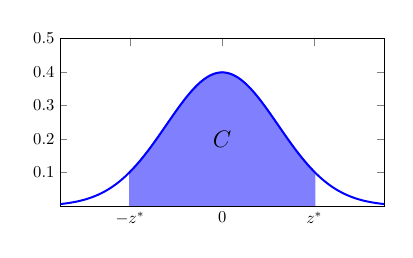
\begin{tikzpicture}[scale = 0.6]
       \begin{axis}[unit vector ratio=1 6 1, ymin=0,ymax=0.5,xmin=-2.9, xmax = 2.9, xtick = {-1.65,0,1.65}, xticklabels = {$-z^*$,$0$,$z^*$}, ytick = {0.1,0.2,0.3,0.4,0.5}]
       \addplot[fill = blue, very thick,domain=-1.65:1.65,blue!50, samples=100] {0.3989*e^(-x^2/2)}\closedcycle;
       \addplot[very thick,domain=-3:3,blue, samples=100] {0.3989*e^(-x^2/2)};
       \addplot[domain=-3:3] {0};
       \node at (axis cs: 0,0.2) {\Large{$C$}};
    \end{axis}
    \end{tikzpicture}
\end{center}
\begin{examp}
The critical value for a confidence level of $90\%$ is $z^* = 1.65$, since $P(-1.65 < Z < 1.65) = P(Z < 1.65) - P(Z < -1.65) = 0.9505 - 0.495 = 0.9$.
\begin{center}
   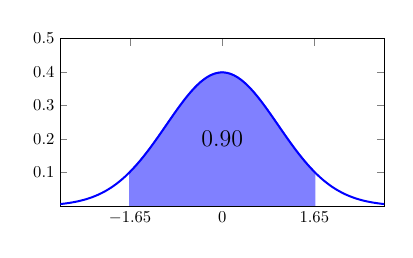
\begin{tikzpicture}[scale = 0.6]
       \begin{axis}[unit vector ratio=1 6 1, ymin=0,ymax=0.5,xmin=-2.9, xmax = 2.9, xtick = {-1.65,0,1.65}, xticklabels = {$-1.65$,$0$,$1.65$}, ytick = {0.1,0.2,0.3,0.4,0.5}]
       \addplot[fill = blue, very thick,domain=-1.65:1.65,blue!50, samples=100] {0.3989*e^(-x^2/2)}\closedcycle;
       \addplot[very thick,domain=-3:3,blue, samples=100] {0.3989*e^(-x^2/2)};
       \addplot[domain=-3:3] {0};
       \node at (axis cs: 0,0.2) {\Large{$0.90$}};
    \end{axis}
    \end{tikzpicture}
\end{center}
When using the $Z$-table, we can find $z^*$ by noting that if $P(-z^* < Z < z^*) = 0.9$, then by symmetry, $P(Z < z^*) = 0.95$. Thus, we're looking for the value of $z$ that has an area of 0.95 to its left.
\end{examp}
\par
If we follow through the calculation we made in the introduction to this section with a general critical value $z^*$ and a general sample mean $\overline{X}$, we'll arrive at a formula for a confidence interval for the mean $\mu$ of any population from which we might draw a sample. With a probability of $C$, we have
\begin{gather*}
-z^* < Z < z^* \\
-z^* < \textstyle\frac{\overline{X}- \muxbar}{\sigmaxbar} < z^* \\
-z^* \sigmaxbar < \overline{X}- \mu < z^* \sigmaxbar \\[0.2ex]
-\overline{X}-z^* \sigmaxbar < - \mu < -\overline{X}+z^* \sigmaxbar \\[0.3ex]
\overline{X}-z^* \sigmaxbar <  \mu < \overline{X}+z^* \sigmaxbar \\[0.3ex]
\overline{X}-z^* \textstyle\frac{\sigma}{\sqrt{n}} <  \mu < \overline{X}+z^* 
\frac{\sigma}{\sqrt{n}}.
\end{gather*}
\par
Note that this calculation only makes sense when $\overline{X}$ is normally distributed, but the Central Limit Theorem tells us this is indeed the case as long as our sample is a SRS of a sufficiently large size. The quantity we add to and subtract from $\overline{X}$ in the last line is called the margin of error.
\begin{defn}\index{Margin of Error} Given a SRS of $n$ values drawn from any distribution and a confidence level $C \in (0,1)$, the margin of error for $\overline{X}$ at confidence level $C$ is 
$$\boxed{E = z^* \frac{\sigma}{\sqrt{n}}}$$
\end{defn}
\par
This value represents the largest possible gap between a sample mean $\overline{X}$ and the population mean $\mu$ that is observed at the confidence level $C$. For example, if $E = 2.2$ when $C = 0.9$, this means there is a $90\%$ probability that a SRS has a mean which differs from the true population mean by less than $2.2$.
\par
With our definitions established, we can describe the procedure for constructing a confidence interval for a population mean $\mu$ based on any SRS of $n$ values with sample mean $\overline{X}$ in three steps.
\begin{enumerate}[(i)]
\item Find the critical value $z^*$ for the desired confidence level $C$.
\item Compute the margin of error $E$.
\vspace*{-0.02in}
\item The confidence interval is given by $\xbar - E < \mu < \xbar + E$.
\end{enumerate}
\begin{example} 
The standard deviation for heights of all men in Canada is known to be around 2.9 inches. In a random sample of 37 Canadian men, the average height was 5'9". Use this information to construct a $95\%$ confidence interval for the average height of all Canadian men.
\par
\noindent The critical value $z^*$ is defined by $P(-z^* < Z < z^*) = 0.95$, so the area on the left of $z^*$ must be $P(Z < z^*) = 0.975$, and consulting the Z-table yields $z^* = 1.96$.
\begin{center}
   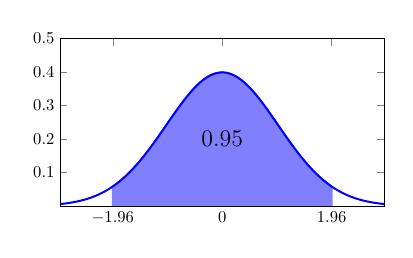
\begin{tikzpicture}[scale = 0.6]
       \begin{axis}[unit vector ratio=1 6 1, ymin=0,ymax=0.5,xmin=-2.9, xmax = 2.9, xtick = {-1.96,0,1.96}, xticklabels = {$-1.96$,$0$,$1.96$}, ytick = {0.1,0.2,0.3,0.4,0.5}]
       \addplot[fill = blue, very thick,domain=-1.96:1.96,blue!50, samples=100] {0.3989*e^(-x^2/2)}\closedcycle;
       \addplot[very thick,domain=-3:3,blue, samples=100] {0.3989*e^(-x^2/2)};
       \addplot[domain=-3:3] {0};
       \node at (axis cs: 0,0.2) {\Large{$0.95$}};
    \end{axis}
    \end{tikzpicture}
\end{center}
\noindent The margin of error is then given by $E = z^*  \frac{\sigma}{\sqrt{n}} = 1.96  \frac{2.9}{\sqrt{37}} \simeq 0.934$. In inches, the sample mean $5'9"$ is $69"$, so we obtain the interval 
$$69-0.934 < \mu < 69+0.934 \ \ \rightarrow \ \ 68.066 < \mu < 69.934$$
\noindent Thus, with $95\%$ confidence, the mean height of all Canadian men must be between 68.066" (about 5'8") and and 69.934" (about 5'10").
\end{example}
\par
Note that when we say `with 95\% confidence, $68.066 < \mu < 69.934$', this means there a 95\% chance that we have selected a sample which will produce a confidence interval containing the true mean height of the population, $\mu$.
\par
The mean height of all Canadian men is some fixed single value, we just don't know what it is. Thus, the probability it's inside our particular confidence interval is either $100\%$ or $0\%$ (it is or it isn't). But if we were to take many random samples and compute a 95\% confidence interval from each, we would expect that, typically, nineteen of every twenty samples would produce intervals that contain the true value of $\mu$ (since 19/20 is 95\%).
\begin{center}
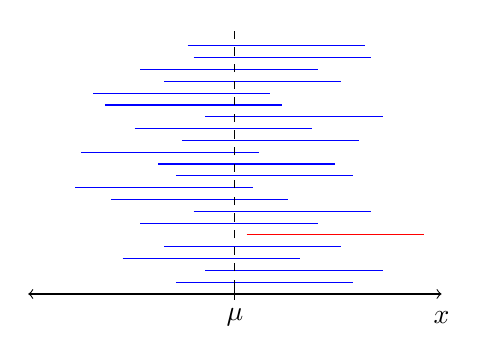
\begin{tikzpicture}[scale=0.75]
\draw[<->] (-3.5,0) -- (3.5,0);
\draw (0,0.1) -- (0,-0.1);
\node at (3.5,-0.4) {$x$};
\node at (0,-0.4) {$\mu$};
\draw[blue] (-1,0.2) -- (2,0.2);
\draw[blue] (-0.5,0.4) -- (2.5,0.4);
\draw[blue] (-1.9,0.6) -- (1.1,0.6);
\draw[blue] (-1.2,0.8) -- (1.8,0.8);
\draw[red] (0.2,1.0) -- (3.2,1.0);
\draw[blue] (-1.6,1.2) -- (1.4,1.2);
\draw[blue] (-0.7,1.4) -- (2.3,1.4);
\draw[blue] (-2.1,1.6) -- (0.9,1.6);
\draw[blue] (-2.7,1.8) -- (0.3,1.8);
\draw[blue] (-1,2.0) -- (2,2.0);
\draw[blue] (-1.3,2.2) -- (1.7,2.2);
\draw[blue] (-2.6,2.4) -- (0.4,2.4);
\draw[blue] (-0.9,2.6) -- (2.1,2.6);
\draw[blue] (-1.7,2.8) -- (1.3,2.8);
\draw[blue] (-0.5,3.0) -- (2.5,3.0);
\draw[blue] (-2.2,3.2) -- (0.8,3.2);
\draw[blue] (-2.4,3.4) -- (0.6,3.4);
\draw[blue] (-1.2,3.6) -- (1.8,3.6);
\draw[blue] (-1.6,3.8) -- (1.4,3.8);
\draw[blue] (-0.7,4.0) -- (2.3,4.0);
\draw[blue] (-0.8,4.2) -- (2.2,4.2);
\draw[dashed] (0,0.1) -- (0,4.5);
\end{tikzpicture}
\end{center}
\par
Notice that as the confidence level becomes larger, the corresponding critical value $z^*$ grows to enclose that larger area, which increases the margin of error, $E$. On the other hand, the value of $E$ is a decreasing function of the sample size, $n$, so a larger sample will lead to a smaller confidence interval, giving a more accurate estimate of the parameter $\mu$.
\begin{prop} To reduce the margin of error, $E$ and produce tighter bounds on $\mu$, we can either decrease the confidence level, $C$, or increase the sample size, $n$.
\end{prop}

\section{Confidence Interval for a Proportion}

What if we're interested in estimating the proportion of individuals in a population that have some property of interest? For example, a pollster might want to estimate the proportion of all voters in some area that intend to vote for a particular political party. We can produce a confidence interval for such a proportion from a random sample using the ideas we developed in the last section.
\par
Each individual in the population either has the desired property or does not, so if the proportion of individuals in the population with the desired property is $p \in [0,1]$ (and hence the proportion without is $1-p$), the population distribution we're interested in is $X \sim Bernoulli(p)$ for some unknown parameter $p$. We'll call $p$ the population proportion. The expected value of its distribution is $E(X) = p$, hence the population mean is also $\mu = p$, as we saw in Section \ref{BernoulliDist}.
\par
Notice that if we sample from a Bernoulli distribution, then the sample mean $\xbar = \frac{1}{n}(X_1+X_2+\cdots+X_n)$ is actually the proportion of individuals in our sample with the desired property (since $X_i$ was drawn from a Bernoulli distribution, so it take the value $1$ when the $i^{th}$ individual has the property, and $0$ if not). Thus, we're counting the number of individuals in our sample with the property and dividing by the sample size, so the sample mean $\xbar$ is in fact equal to the sample proportion in this context. To remind ourselves it's a proportion we can write $\widehat{p} = \xbar$.
\par
In summary, if our population distribution is $X \sim Bernoulli(p)$, then the population mean and sample mean are equal to the population proportion and sample proportion respectively, that is, $p = \mu$, and $\widehat{p}=\xbar$. This means we can construct confidence intervals for a proportion in exactly the same way we made confidence intervals for the mean in the last section.
\par
In Section \ref{BernoulliDist}, we saw that the variance of a Bernoulli distribution is given by the formula $\sigma^2 = p(1-p)$, so the margin of error $E$ becomes
$$E = z^*  \frac{\sigma}{\sqrt{n}} = z^*  \frac{\sqrt{p(1-p)}}{\sqrt{n}}$$
and although we can't know the value of $\sqrt{p(1-p)}$ (because $p$ is the unknown we're trying to estimate), we can bound it.
\begin{prop} If $p \in [0,1]$, then $0 \leq \sqrt{p(1-p)} \leq \frac{1}{2}$, and therefore the margin of error for a sample proportion $\widehat{p}$ satisfies
$$\boxed{E \leq z^*  \frac{1}{2\sqrt{n}}}$$
\end{prop}
\begin{pf} Define $f(p) = p(1-p)$. Notice that to max/minimize $\sqrt{p(1-p)}$ on $[0,1]$, we can max/minimize $f(p)$ on $[0,1]$. Since $f$ is continuous and differentiable on $[0,1]$, it will attain its max/minimum values at a critical point or at an endpoint.
$$f'(p) = (1)(1-p) + (p)(-1) = 1 - 2p$$
Therefore, the only critical point of $f$ is $p = \frac{1}{2}$. Evaluating $f$ at this point and the two endpoints of $[0,1]$ yields
\vspace*{-0.1in}
\begin{center}
\def\arraystretch{1.5}%
\begin{tabular}{c|c}
$p$ \ & $f(p)$ \\
\hline
$0$ \ & $0$ \\
$\frac{1}{2}$ \ & $\frac{1}{4}$ \\
$1$ \ & $0$ \\
\end{tabular}
\end{center}
\vspace*{-0.05in}
Therefore, $f$ attains its maximum value at $p = \frac{1}{2}$, and hence
$$E = z^*   \frac{\sqrt{p(1-p)}}{\sqrt{n}} \leq z^*  \frac{\sqrt{\frac{1}{2}(1 -\frac{1}{2})}}{\sqrt{n}} = z^*  \frac{1}{2\sqrt{n}}$$
\end{pf}
\par
We can use this result to construct confidence intervals for a population proportion, but keep in mind we have an upper bound, not the true value of $E$. When we construct a $95\%$ confidence interval, there should be a $95\%$ probability of selecting a sample that results in an interval containing the parameter we're estimating. If we use the bound on $E$ that was just derived, this probability may in fact be larger than $95\%$, that is, our interval will generally be be wider than is necessary.
\par
\begin{examp}Suppose that a pollster is interested in knowing what proportion of voters in a certain riding plan to vote NDP. In a random sample of 817 voters from this riding, 227 plan to vote NDP. Construct a $92\%$ confidence interval for the proportion of all voters in this riding who plan to vote NDP.
\par
\noindent The critical value $z^*$ is defined by $P(-z^* < Z < z^*) = 0.92$, so the area on the left of $z^*$ must be $P(Z < z^*) = 0.96$, and consulting the Z-table yields $z^* = 1.75$.
\begin{center}
   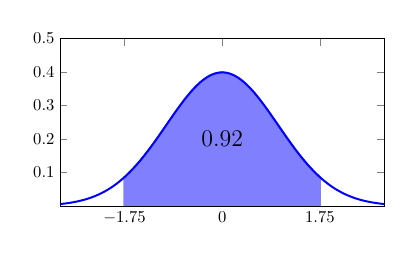
\begin{tikzpicture}[scale = 0.6]
       \begin{axis}[unit vector ratio=1 6 1, ymin=0,ymax=0.5,xmin=-2.9, xmax = 2.9, xtick = {-1.75,0,1.75}, xticklabels = {$-1.75$,$0$,$1.75$}, ytick = {0.1,0.2,0.3,0.4,0.5}]
       \addplot[fill = blue, very thick,domain=-1.75:1.75,blue!50, samples=100] {0.3989*e^(-x^2/2)}\closedcycle;
       \addplot[very thick,domain=-3:3,blue, samples=100] {0.3989*e^(-x^2/2)};
       \addplot[domain=-3:3] {0};
       \node at (axis cs: 0,0.2) {\Large{$0.92$}};
    \end{axis}
    \end{tikzpicture}
\end{center}
\noindent The margin of error satisfies $E \leq z^*  \frac{1}{2\sqrt{n}} = 1.75 \frac{1}{2\sqrt{817}} \simeq 0.031$, and since the sample proportion is $\widehat{p} = \frac{227}{817} = 0.278$, we have
$$0.278-0.031 < p < 0.278+0.031 \ \ \rightarrow \ \ 0.247 < p < 0.309.$$
\noindent Thus, with $95\%$ confidence, the proportion of voters in the riding who plan to vote NDP is between $24.7\%$ and $30.9\%$.
\end{examp}
\par
Note that if you look up the margin of error formula for estimating a proportion in other sources you'll likely encounter the formula $$E = z^*\sqrt{\frac{\widehat{p}(1-\widehat{p})}{n}}.$$
This is the same error bound we derived at the beginning of this section, but the unknown population proportion $p$ has been replaced by the sample proportion $\widehat{p}$. As the sample size increases, we know $\widehat{p} \rightarrow p$ by the law of large numbers, but for any fixed $n$, they will differ, so to properly justify this error bound requires more work, as this difference introduces a new source of uncertainty we have not quantified.

\section{Confidence Interval for a Mean ($\sigma$ Unknown)}

Our procedure for constructing a confidence interval for a population mean $\mu$ requires knowledge of the population standard deviation $\sigma$. This is to be expected, as means of samples from a population with a large standard deviation will be more variable more than means of samples from a population with a low standard deviation. Unfortunately, this requirement is problematic in practice since $\sigma$ is a parameter of the population distribution, so is typically unknown.
\par
We got around this requirement when estimating a proportion by establishing an upper bound on the population standard deviation $\sigma = \sqrt{p(1-p)}$, but no such upper bound exists in general when we're estimating a mean.
\par
If we can't find an upper bound the value of $\sigma$, can we estimate it in some other way? Well, the best estimate of the population we have access to is our sample, so what if we simply use the standard deviation of our sample in place of the standard deviation of the population?
\par
\begin{defn}\index{Sample Standard Deviation}\index{Standard Deviation! of a sample}\index{Bessel's Correction}\label{SampleStdDev}The (Bessel corrected) sample variance is $S^2 = \frac{1}{n-1}\sum_{i} (X_i - \overline{X})^2$ and the sample standard deviation, $S$, is the square root of the sample variance.
\end{defn}
\par
\begin{examp} Find the mean and standard deviation of the sample of five values $X_1 = 2$, $X_2 = 0$, $X_3 = 7$, $X_4 = 3$, $X_5 = 3$, drawn from an unknown distribution.

$$\xbar = \textstyle\frac{1}{n}\sum_{i} X_i = \frac{1}{5}(2+0+7+3+3) = 3$$
$$S = \textstyle\sqrt{\frac{1}{n-1}\sum_{i} (X_i - \overline{X})^2} = \textstyle\sqrt{\frac{1}{4}((-1)^2+(-3)^2+(4)^2+(0)^2+(0)^2)} = \textstyle\sqrt{\frac{13}{2}}$$
\end{examp}
\par
Note that when calculating $S^2$ and $S$, we don't divide by the sample size, $n$, as in Definition \ref{VarianceDef}, but instead by $n-1$. This change is known as Bessel's correction, and it's done to obtain an unbiased estimator of the population variance. The formula in Definition \ref{VarianceDef} systematically underestimates the population variance.
\begin{thm}The Bessel corrected sample variance $S^2 = \frac{1}{n-1}\sum_{i} (X_i - \overline{X})^2$, is an unbiased estimator of the population variance, that is, $E(S^2) = \sigma^2$.
\end{thm} 
\begin{pf} This follows from a long and careful calculation using properties of expected value. One key fact to recall is that $\Var(X) = E[X^2] - (E[X])^2$ for any random variable $X$, and hence $E[X^2] = Var(X) + (E[X])^2$.
\eqnsgap{E(S^2) &= E\left(\textstyle\frac{1}{n-1}\displaystyle \sum_{i} (X_i - \overline{X})^2 \right) \\
&= \textstyle\frac{1}{n-1}\displaystyle E\left(\sum_{i} (X_i - \xbar)^2\right) \\
&= \textstyle\frac{1}{n-1}\displaystyle E\left(\sum_{i} \left(X_i^2 - 2X_i\xbar + \xbar^2\right)\right) \\
&= \textstyle\frac{1}{n-1}\displaystyle E\left(\sum_{i}X_i^2 - \sum_{i}2X_i\xbar + \sum_{i}\xbar^2\right) \\}
\eqnsgap{\hspace*{1.275in}&= \textstyle\frac{1}{n-1}\displaystyle E\left(\sum_{i}X_i^2 - 2\xbar\sum_{i}X_i + n\xbar^2\right) \\
&= \textstyle\frac{1}{n-1}\displaystyle E\left(\sum_{i}X_i^2 - 2\xbar\cdot n\xbar + n\xbar^2\right) \\
&= \textstyle\frac{1}{n-1}\displaystyle E\left(\sum_{i}X_i^2 - n\xbar^2\right) \\
&= \textstyle\frac{1}{n-1}\displaystyle \left(\sum_{i}E[X_i^2] - E[n\xbar^2]\right) \\
&= \textstyle\frac{1}{n-1}\displaystyle \left(nE[X^2] - nE[\xbar^2]\right) \\
&= \textstyle\frac{1}{n-1}\displaystyle \biggr(n(Var(X) + (E[X])^2) - n(Var(\xbar)+(E[\xbar])^2)\biggr)\\
&= \textstyle\frac{1}{n-1}\displaystyle \left(n(\sigma^2 + \mu^2) - n(\textstyle\frac{\sigma^2}{n}+\mu^2)\right) \\
&= \textstyle\frac{1}{n-1}\displaystyle \left(n\sigma^2 + n\mu^2 - \sigma^2 -n\mu^2\right) \\
&= \textstyle\frac{1}{n-1}\displaystyle \left((n-1)\sigma^2\right) = \sigma^2}
\end{pf}

In practice, Bessel's correction is used almost universally. Try calculating the standard deviation of a small list of values using a spreadsheet on a computer. Is the calculation done with or without Bessel's correction?
\par
If we use the sample standard deviation, $s$, to estimate the standard deviation in our population, $\sigma$, then when we standardize a sample mean $\xbar$, instead of the standardized value
$$\frac{\overline{X} - \muxbar}{\sigmaxbar} = \frac{\overline{X} - \mu}{\frac{\sigma}{\sqrt{n}}}, \ \ \text{we'll have the estimate} \ \ \frac{\overline{X} - \muxbar}{\sigmaxbar} \simeq \frac{\overline{X} - \mu}{\frac{S}{\sqrt{n}}}.$$
Our construction of a confidence interval for the population mean $\mu$ was justified by the Central Limit Theorem, which tells us the distribution of the quantity on the left approaches $Z \sim Normal(0,1)$ as the sample size $n$ grows (and is exactly equal to $Z \sim Normal(0,1)$ when the population distribution is normal). But what about our estimate on the right? If we repeatedly draw samples and calculate this value, what kind of distribution will we obtain?
\par
\begin{defn}\label{TDistDef}\index{T-distribution} Suppose we draw a SRS $X_1, X_2, \, \dots \, , X_n$ from a normally distributed population with mean $\mu$, and define the $T$-score of the sample as
$$T = \frac{\overline{X} - \mu}{\frac{S}{\sqrt{n}}}$$
where $S$ is the sample standard deviation, as in Definition \ref{SampleStdDev}. Then $T$ is a continuous random variable whose distribution is called Student's $T$-distribution (or simply the $T$-distribution) with $n-1$ degrees of freedom.
\end{defn}
%gnuplot is used to draw t-distributions.
\begin{center}
\begin{tikzpicture}[scale = 0.65]
\begin{axis}[ymin=0,ymax=0.42,xmin=-3, xmax = 3, xtick = {-2,-1,0,1,2}, ytick = {}]
       \addplot[very thick,domain=-3:3,blue,samples=100] gnuplot {(gamma(1)/(sqrt(pi)*gamma(0.5)))*(1+x*x)**(-1)};
       \addplot[very thick,domain=-3:3,blue,samples=100, opacity=0.8] gnuplot {(gamma(1.5)/(sqrt(2*pi)*gamma(1)))*(1+(0.5)*x*x)**(-(1.5))};
       \addplot[very thick,domain=-3:3,blue,samples=100, opacity=0.6] gnuplot {(gamma(0.5*(4+1))/(sqrt(4*pi)*gamma((0.5*4))))*(1+(0.25)*x*x)**(-(0.5*(4+1)))};
       \addplot[very thick,domain=-3:3,blue,samples=100, opacity=0.4] gnuplot {(gamma(0.5*(10+1))/(sqrt(10*pi)*gamma((0.5*10))))*(1+(0.1)*x*x)**(-(0.5*(10+1)))};
       \addplot[very thick,domain=-3:3,blue,samples=100, opacity=0.2] gnuplot {(gamma(0.5*(100+1))/(sqrt(100*pi)*gamma((0.5*100))))*(1+(0.01)*x*x)**(-(0.5*(100+1)))};
       \addplot[very thick,domain=-3:3,black,dashed,samples=100] {0.3989*e^(-x^2/2)};
\end{axis}
\end{tikzpicture}
\end{center}
\par
Above in blue are plots of probability density functions for $T$-distributions with one, two, four, ten, and one hundred degrees of freedom, shaded lighter as the degree of freedom grows. The standard normal distribution is shown in dashed black.
\par 
The $T$-distribution has fatter tails and less area near the center than the standard normal distribution. This additional variability appears because the sample standard deviation $S$ differs from one sample to the next, which adds a source of variability to $T$-scores which is not present in $Z$-scores. As the sample size grows, the sample standard deviation $S$ becomes a better estimator of the population standard deviation $\sigma$, and the $T$-distribution slowly approaches the standard normal distribution. Notice that once the degree of freedom reaches one hundred, the $T$-distribution and the standard normal distribution are effectively identical.
\par
If we can find areas under the $T$-distribution, then the same procedure we've been using to construct confidence intervals with the population standard deviation can be modified to work with the sample standard deviation.
\begin{prop}Let $T$ be a random variable whose distribution is the $T$ distribution with $n-1$ degrees of freedom, and take $t^*$ so that $P(-t^* < T < t^*) = C$.
\par
\noindent If we define $E = t^*\frac{S}{\sqrt{n}}$, then $P(\mu \in (\xbar - E, \xbar + E)) = C$, where $\xbar$ is the mean of a SRS drawn from a normal distribution with mean $\mu$.
\end{prop}
\begin{pf}
By definition of $t^*$, with probability $C$ we have
\begin{gather*}
-t^* < T < t^* \\
-t^* < \textstyle\frac{\overline{X}- \mu}{\frac{S}{\sqrt{n}}} < t^* \\
-t^* \textstyle\frac{S}{\sqrt{n}} < \overline{X}- \mu < t^* \frac{S}{\sqrt{n}} \\[0.2ex]
-\overline{X}-t^* \textstyle\frac{S}{\sqrt{n}} < - \mu < -\overline{X}+t^* \frac{S}{\sqrt{n}} \\[0.3ex]
\overline{X}-t^* \textstyle\frac{S}{\sqrt{n}} <  \mu < \overline{X}+t^* \frac{S}{\sqrt{n}}.
\end{gather*}
\end{pf}
\par
\begin{examp}\label{TIntExample} A sample of five values is drawn from a normal distribution with unknown mean and standard deviation. These values are $43$, $27$, $30$, $22$, and $38$. Construct a 90\% confidence interval for the mean of the normal distribution.
\par
\noindent Computing the mean and (Bessel corrected) standard deviation of the sample yields $\xbar = 32$ and $S = 8.456$. We can now construct a confidence interval for the population mean $\mu$ just as we've done before in Section \ref{ConfIntervalMeanSec}, but using $s$ in place of $\sigma$ and the $T$-distribution in place of the standard normal distribution.
\begin{center}
   \begin{tikzpicture}[scale = 0.6]
       \begin{axis}[unit vector ratio=1 6 1, ymin=0,ymax=0.5,xmin=-2.9, xmax = 2.9, xtick = {-2.13,0,2.13}, xticklabels = {$-2.13$,$0$,$2.13$}, ytick = {0.1,0.2,0.3,0.4,0.5}]
       \addplot[fill = blue, very thick,domain=-2.13:2.13,blue!50, samples=100]  gnuplot {(gamma(0.5*(4+1))/(sqrt(4*pi)*gamma((0.5*4))))*(1+(0.25)*x*x)**(-(0.5*(4+1)))}\closedcycle;
       \addplot[very thick,domain=-3:3,blue, samples=100]  gnuplot {(gamma(0.5*(4+1))/(sqrt(4*pi)*gamma((0.5*4))))*(1+(0.25)*x*x)**(-(0.5*(4+1)))};
       \addplot[domain=-3:3] {0};
       \node at (axis cs: 0,0.2) {\Large{$0.9$}};
    \end{axis}
    \end{tikzpicture}
\end{center}
\noindent We compute $t^* = 2.13$ using a table of values for the $t$-distribution (with 4 degrees of freedom), then $E = t^{*} \frac{s}{\sqrt{n}} = 2.13 \cdot \frac{8.456}{\sqrt{5}} = 8.05$, and therefore with $90\%$ confidence we have
$$32 - 8.05 < \mu < 32 + 8.05 \ \ \rightarrow \ \ 23.95 < \mu < 40.05$$
\end{examp}

\subsection*{Robustness}
Notice that the $T$-distribution is defined as the distribution of $T$-scores of random samples drawn from a normal distribution. In practice though, we would rarely know enough about the population we are studying to be able to determine if the random variable whose mean we want to estimate is normally distributed.
\par
Fortunately, whenever the hypotheses of the central limit theorem hold, the distribution of $T$-scores of random samples drawn from any distribution will, in fact, eventually converge to the $T$-distribution \cite{AsymptoticTDist} as the sample size grows larger. 
\par
Even with smaller sample sizes, statisticians like to say that the confidence interval procedure above in Example \ref{TIntExample} is `robust to non-normality'. This means that although the assumption that we're sampling from a normal distribution is necessary for strict correctness of the procedure, bending the rules on this assumption will typically introduce only a small source of error. However, with small samples from a population whose distribution is not known to be bell-shaped, one can be justifiably suspicious, especially if there's reason to believe the distribution of the population could be fat-tailed or very asymmetric.
\par
\begin{examp}
In a study of a particular species of maple in a provincial park, the height of every tree in a random sample of 38 mature trees was measured. If the sample mean and sample standard deviation for the heights of the trees were $21.3$ metres and $4.9$ metres respectively, construct a $90\%$ confidence interval for the mean height of all trees of this species in the park.
\par
\noindent We have $\xbar = 21.3$, $S = 4.9$, and $n = 38$. Using the $T$-table, we can see that in a $T$-distribution with 37 degrees of freedom, $P(-1.69 < T < 1.69) = 0.9$, so the critical value is $t^* = 1.69$.
\par
\noindent
We can then compute the margin of error $E = t^* \frac{s}{\sqrt{n}} = 1.69 \frac{4.9}{\sqrt{38}} = 1.343$, and write the confidence interval
$$21.3-1.343 < \mu < 21.3+1.343 \ \ \rightarrow \ \ 19.957 < \mu < 22.643.$$
Therefore, with $90\%$ confidence, the mean height of all mature trees of this species in the park is between $19.9$ and $22.7$ metres.
\end{examp}
\par
In examples like the one above, where the distribution our sample is drawn from is somewhat bell-shaped, without fat tails (think about what kind of shape the distribution of heights of mature trees might have), confidence intervals constructed using the $T$-distribution are typically very accurate for all but extremely small sample sizes.








